\chapter{AFABL: A Friendly Adaptive Behavior Language}\label{ch:afabl}

PLACEHOLDER PLACEHOLDER PLACEHOLDER PLACEHOLDER PLACEHOLDER PLACEHOLDER PLACEHOLDER PLACEHOLDER PLACEHOLDER PLACEHOLDER PLACEHOLDER PLACEHOLDER PLACEHOLDER PLACEHOLDER PLACEHOLDER PLACEHOLDER PLACEHOLDER PLACEHOLDER PLACEHOLDER PLACEHOLDER PLACEHOLDER PLACEHOLDER PLACEHOLDER PLACEHOLDER PLACEHOLDER PLACEHOLDER PLACEHOLDER PLACEHOLDER PLACEHOLDER PLACEHOLDER PLACEHOLDER PLACEHOLDER PLACEHOLDER PLACEHOLDER PLACEHOLDER PLACEHOLDER PLACEHOLDER PLACEHOLDER PLACEHOLDER PLACEHOLDER PLACEHOLDER PLACEHOLDER PLACEHOLDER PLACEHOLDER PLACEHOLDER PLACEHOLDER PLACEHOLDER PLACEHOLDER

\section{Background}

PLACEHOLDER PLACEHOLDER PLACEHOLDER PLACEHOLDER PLACEHOLDER PLACEHOLDER PLACEHOLDER PLACEHOLDER PLACEHOLDER PLACEHOLDER PLACEHOLDER PLACEHOLDER PLACEHOLDER PLACEHOLDER PLACEHOLDER PLACEHOLDER PLACEHOLDER PLACEHOLDER PLACEHOLDER PLACEHOLDER PLACEHOLDER PLACEHOLDER PLACEHOLDER PLACEHOLDER PLACEHOLDER PLACEHOLDER PLACEHOLDER PLACEHOLDER PLACEHOLDER PLACEHOLDER PLACEHOLDER PLACEHOLDER PLACEHOLDER PLACEHOLDER PLACEHOLDER PLACEHOLDER PLACEHOLDER PLACEHOLDER PLACEHOLDER PLACEHOLDER PLACEHOLDER PLACEHOLDER PLACEHOLDER PLACEHOLDER PLACEHOLDER PLACEHOLDER PLACEHOLDER PLACEHOLDER

\subsection{Why an Embedded Domain-Specific Language?}

PLACEHOLDER PLACEHOLDER PLACEHOLDER PLACEHOLDER PLACEHOLDER PLACEHOLDER PLACEHOLDER PLACEHOLDER PLACEHOLDER PLACEHOLDER PLACEHOLDER PLACEHOLDER PLACEHOLDER PLACEHOLDER PLACEHOLDER PLACEHOLDER PLACEHOLDER PLACEHOLDER PLACEHOLDER PLACEHOLDER PLACEHOLDER PLACEHOLDER PLACEHOLDER PLACEHOLDER PLACEHOLDER PLACEHOLDER PLACEHOLDER PLACEHOLDER PLACEHOLDER PLACEHOLDER PLACEHOLDER PLACEHOLDER PLACEHOLDER PLACEHOLDER PLACEHOLDER PLACEHOLDER PLACEHOLDER PLACEHOLDER PLACEHOLDER PLACEHOLDER PLACEHOLDER PLACEHOLDER PLACEHOLDER PLACEHOLDER PLACEHOLDER PLACEHOLDER PLACEHOLDER PLACEHOLDER

\subsection{Why Scala?}

PLACEHOLDER PLACEHOLDER PLACEHOLDER PLACEHOLDER PLACEHOLDER PLACEHOLDER PLACEHOLDER PLACEHOLDER PLACEHOLDER PLACEHOLDER PLACEHOLDER PLACEHOLDER PLACEHOLDER PLACEHOLDER PLACEHOLDER PLACEHOLDER PLACEHOLDER PLACEHOLDER PLACEHOLDER PLACEHOLDER PLACEHOLDER PLACEHOLDER PLACEHOLDER PLACEHOLDER PLACEHOLDER PLACEHOLDER PLACEHOLDER PLACEHOLDER PLACEHOLDER PLACEHOLDER PLACEHOLDER PLACEHOLDER PLACEHOLDER PLACEHOLDER PLACEHOLDER PLACEHOLDER PLACEHOLDER PLACEHOLDER PLACEHOLDER PLACEHOLDER PLACEHOLDER PLACEHOLDER PLACEHOLDER PLACEHOLDER PLACEHOLDER PLACEHOLDER PLACEHOLDER PLACEHOLDER

\section{AFABL Concepts}

PLACEHOLDER PLACEHOLDER PLACEHOLDER PLACEHOLDER PLACEHOLDER PLACEHOLDER PLACEHOLDER PLACEHOLDER PLACEHOLDER PLACEHOLDER PLACEHOLDER PLACEHOLDER PLACEHOLDER PLACEHOLDER PLACEHOLDER PLACEHOLDER PLACEHOLDER PLACEHOLDER PLACEHOLDER PLACEHOLDER PLACEHOLDER PLACEHOLDER PLACEHOLDER PLACEHOLDER PLACEHOLDER PLACEHOLDER PLACEHOLDER PLACEHOLDER PLACEHOLDER PLACEHOLDER PLACEHOLDER PLACEHOLDER PLACEHOLDER PLACEHOLDER PLACEHOLDER PLACEHOLDER PLACEHOLDER PLACEHOLDER PLACEHOLDER PLACEHOLDER PLACEHOLDER PLACEHOLDER PLACEHOLDER PLACEHOLDER PLACEHOLDER PLACEHOLDER PLACEHOLDER PLACEHOLDER

\subsection{Terminology}

\begin{itemize}

\item State

  A state is a configuration of all objects and agents in a world.
  These configurations can include object locations and orientations,
  mental or emotional dispositions of agents, or indications of the
  occurrence of events (e.g., agent X just got shot).

\item Perception, or Percept

  A subset of a world state that is perceived by an agent.

\item Action

  An action is a one-shot state manipulation that can be executed by
  an agent.  Sometimes called "primitives," actions acquire greater
  meaning when they are executed (possibly in sequences) by behavior
  modules to achieve a goal or satisfy a constraint.


\item World

  Sometimes called an "environment," a world is a container for all
  the things an agent can perceive and act upon, and possibly hidden
  things.  Worlds are represented by states that specify the
  configuration of all the things in a world at a given point in time.

\item World Dynamics

  The dynamics of a world specifies the state transitions that are
  made in response to the execution of actions.  World dynamics may be
  deterministic or stochastic.  Markov Decision Processes are often
  used to represent world dynamics.

\item Behavior Module

  A behavior module is a self-contained agent component that
  recommends an action (response) for a given state perception
  (stimulus).  Anything that produces a policy (a mapping from states
  to actions and tasks) is a behavior module.  A behavior module is
  sometimes called a "subagent" in modular reinforcement learning.

\item Agent

  An agent is an entity that acts under its own control, perceiving
  the state of its world and executing actions in response to these
  perceived states.

\item Intelligent Agent

  An intelligent agent is an agent that chooses its actions to achieve
  goals or satisfy constraints.

\item Adaptive Agent

  An adaptive agent is an intelligent agent that can automatically
  adapt its behaviors to different worlds (that is, choose different
  actions sequences to achieve goals in worlds with different
  dynamics), or adapt its behaviors at run-time to worlds in which the
  dynamics change.

\item Modular Agent

  A modular agent is an agent that consists of multiple behavior
  modules and performs command arbitration to decide which module's
  preferred action to execute in a given state.

\item Command Arbitration

  Command arbitration is the act of deciding, for a given state, which
  behavior module's preferred action to execute in a given state.
\end{itemize}

\subsection{Agent Architecture}

An AFABL agent is a behavorial agent that is composed of reusable
behavior modules.  By "behavioral agent" we mean that the agent
executes an action in resopnse to a stimulus, represented by a state
observation.  Each behavior module is itself an agent that has a
preferred action for each state.  AFABL agents perform command
arbitration to choose one of the modules' recommended actions for each
state.  The behavior modules recommend actions in each state, and the
arbitrator chooses which module to "listen to" in each state.  The
AFABL agent architecture is a subsumption architecture.

\subsubsection{Behavior Modules}

Behavior modules, sometimes called subagents in the modular
reinforcement learning iterature, are agents that are meant to be
combined to form larger agents.  Behavior modules are similar to the
layers of Brooks's subsumption architecture with an important
difference: autonomy.  The internal working of a behavior module is
never altered externally.  A behavior module defines a state
abstraction that converts the state observation it is given to a
(possibly) simpler state that is used internally for decision making
and learning.  The decision making and adaptation mechanisms inside a
module remain completely under the module's control.  Interaction with
the module consists entirely of reporting a state observation to the
module, asking the module for an action, and reporting to the module
the effect of executing an action.

\subsubsection{Adaptive Modules}

An adaptive module employs learning algorithms under the hood to
achieve automatic adaptivity.  By adaptive we mean two things: (1)
adaptation to new worlds, and (2) run-time adaptaion.  A module that
is programmed to work for worlds with a given state representation
will work with any world that provides the same (or greater) state
representation, even if the dynamics of the worlds differ.  An
adaptive module need simply be retrained for the new world.  Once an
adaptive module is running in an active agent, the module may continue
to tune its internal learning models as the agent acts in the world,
providing for run-time adaptation.

\subsubsection{Command Arbitrators}

Command arbitrators take as input the action preferences of a set of
modules, and selects one of the actions.  If the command arbitrator is
part of a module, the action selected is the preferred action of the
module.  If the command arbitrator is part of the top-level agent,
then the actoin selected is the action that will be executed by the
agent.

\subsection{Reinforcement Learning in AFABL}

PLACEHOLDER PLACEHOLDER PLACEHOLDER PLACEHOLDER PLACEHOLDER PLACEHOLDER PLACEHOLDER PLACEHOLDER PLACEHOLDER PLACEHOLDER PLACEHOLDER PLACEHOLDER PLACEHOLDER PLACEHOLDER PLACEHOLDER PLACEHOLDER PLACEHOLDER PLACEHOLDER PLACEHOLDER PLACEHOLDER PLACEHOLDER PLACEHOLDER PLACEHOLDER PLACEHOLDER PLACEHOLDER PLACEHOLDER PLACEHOLDER PLACEHOLDER PLACEHOLDER PLACEHOLDER PLACEHOLDER PLACEHOLDER PLACEHOLDER PLACEHOLDER PLACEHOLDER PLACEHOLDER PLACEHOLDER PLACEHOLDER PLACEHOLDER PLACEHOLDER PLACEHOLDER PLACEHOLDER PLACEHOLDER PLACEHOLDER PLACEHOLDER PLACEHOLDER PLACEHOLDER PLACEHOLDER

\section{The AFABL Language}

PLACEHOLDER PLACEHOLDER PLACEHOLDER PLACEHOLDER PLACEHOLDER PLACEHOLDER PLACEHOLDER PLACEHOLDER PLACEHOLDER PLACEHOLDER PLACEHOLDER PLACEHOLDER PLACEHOLDER PLACEHOLDER PLACEHOLDER PLACEHOLDER PLACEHOLDER PLACEHOLDER PLACEHOLDER PLACEHOLDER PLACEHOLDER PLACEHOLDER PLACEHOLDER PLACEHOLDER PLACEHOLDER PLACEHOLDER PLACEHOLDER PLACEHOLDER PLACEHOLDER PLACEHOLDER PLACEHOLDER PLACEHOLDER PLACEHOLDER PLACEHOLDER PLACEHOLDER PLACEHOLDER PLACEHOLDER PLACEHOLDER PLACEHOLDER PLACEHOLDER PLACEHOLDER PLACEHOLDER PLACEHOLDER PLACEHOLDER PLACEHOLDER PLACEHOLDER PLACEHOLDER PLACEHOLDER

\subsection{Worlds}

Every AFABL module and agent is designed to operate in a world. AFABL does not offer any special syntax for creating worlds. Worlds are defined using standard Scala.

\subsubsection{States}

\begin{figure}[ht]
\begin{center}

\begin{lstlisting}[language=Scala]
case class Location(x: Int, y: Int)

case class BunnyState(
  bunny: Location,
  wolf: Location,
  food: Location
)
\end{lstlisting}

\caption{}
\end{center}
\label{fig:bunny-action-code}
\end{figure}


PLACEHOLDER PLACEHOLDER PLACEHOLDER PLACEHOLDER PLACEHOLDER PLACEHOLDER PLACEHOLDER PLACEHOLDER PLACEHOLDER PLACEHOLDER PLACEHOLDER PLACEHOLDER PLACEHOLDER PLACEHOLDER PLACEHOLDER PLACEHOLDER PLACEHOLDER PLACEHOLDER PLACEHOLDER PLACEHOLDER PLACEHOLDER PLACEHOLDER PLACEHOLDER PLACEHOLDER PLACEHOLDER PLACEHOLDER PLACEHOLDER PLACEHOLDER PLACEHOLDER PLACEHOLDER PLACEHOLDER PLACEHOLDER PLACEHOLDER PLACEHOLDER PLACEHOLDER PLACEHOLDER PLACEHOLDER PLACEHOLDER PLACEHOLDER PLACEHOLDER PLACEHOLDER PLACEHOLDER PLACEHOLDER PLACEHOLDER PLACEHOLDER PLACEHOLDER PLACEHOLDER PLACEHOLDER

\subsubsection{Actions}

\begin{figure}[ht]
\begin{center}

\begin{lstlisting}[language=Scala]
object BunnyAction extends Enumeration {
  type BunnyAction = Value
  val Up = Value("^")
  val Down = Value("v")
  val Left = Value("<")
  val Right = Value(">")
}
\end{lstlisting}

\caption{}
\end{center}
\label{fig:bunny-action-code}
\end{figure}


PLACEHOLDER PLACEHOLDER PLACEHOLDER PLACEHOLDER PLACEHOLDER PLACEHOLDER PLACEHOLDER PLACEHOLDER PLACEHOLDER PLACEHOLDER PLACEHOLDER PLACEHOLDER PLACEHOLDER PLACEHOLDER PLACEHOLDER PLACEHOLDER PLACEHOLDER PLACEHOLDER PLACEHOLDER PLACEHOLDER PLACEHOLDER PLACEHOLDER PLACEHOLDER PLACEHOLDER PLACEHOLDER PLACEHOLDER PLACEHOLDER PLACEHOLDER PLACEHOLDER PLACEHOLDER PLACEHOLDER PLACEHOLDER PLACEHOLDER PLACEHOLDER PLACEHOLDER PLACEHOLDER PLACEHOLDER PLACEHOLDER PLACEHOLDER PLACEHOLDER PLACEHOLDER PLACEHOLDER PLACEHOLDER PLACEHOLDER PLACEHOLDER PLACEHOLDER PLACEHOLDER PLACEHOLDER

\subsection{Modules}

PLACEHOLDER PLACEHOLDER PLACEHOLDER PLACEHOLDER PLACEHOLDER PLACEHOLDER PLACEHOLDER PLACEHOLDER PLACEHOLDER PLACEHOLDER PLACEHOLDER PLACEHOLDER PLACEHOLDER PLACEHOLDER PLACEHOLDER PLACEHOLDER PLACEHOLDER PLACEHOLDER PLACEHOLDER PLACEHOLDER PLACEHOLDER PLACEHOLDER PLACEHOLDER PLACEHOLDER PLACEHOLDER PLACEHOLDER PLACEHOLDER PLACEHOLDER PLACEHOLDER PLACEHOLDER PLACEHOLDER PLACEHOLDER PLACEHOLDER PLACEHOLDER PLACEHOLDER PLACEHOLDER PLACEHOLDER PLACEHOLDER PLACEHOLDER PLACEHOLDER PLACEHOLDER PLACEHOLDER PLACEHOLDER PLACEHOLDER PLACEHOLDER PLACEHOLDER PLACEHOLDER PLACEHOLDER

\subsection{Agents}

PLACEHOLDER PLACEHOLDER PLACEHOLDER PLACEHOLDER PLACEHOLDER PLACEHOLDER PLACEHOLDER PLACEHOLDER PLACEHOLDER PLACEHOLDER PLACEHOLDER PLACEHOLDER PLACEHOLDER PLACEHOLDER PLACEHOLDER PLACEHOLDER PLACEHOLDER PLACEHOLDER PLACEHOLDER PLACEHOLDER PLACEHOLDER PLACEHOLDER PLACEHOLDER PLACEHOLDER PLACEHOLDER PLACEHOLDER PLACEHOLDER PLACEHOLDER PLACEHOLDER PLACEHOLDER PLACEHOLDER PLACEHOLDER PLACEHOLDER PLACEHOLDER PLACEHOLDER PLACEHOLDER PLACEHOLDER PLACEHOLDER PLACEHOLDER PLACEHOLDER PLACEHOLDER PLACEHOLDER PLACEHOLDER PLACEHOLDER PLACEHOLDER PLACEHOLDER PLACEHOLDER PLACEHOLDER

\subsubsection{Command Arbitrators}

PLACEHOLDER PLACEHOLDER PLACEHOLDER PLACEHOLDER PLACEHOLDER PLACEHOLDER PLACEHOLDER PLACEHOLDER PLACEHOLDER PLACEHOLDER PLACEHOLDER PLACEHOLDER PLACEHOLDER PLACEHOLDER PLACEHOLDER PLACEHOLDER PLACEHOLDER PLACEHOLDER PLACEHOLDER PLACEHOLDER PLACEHOLDER PLACEHOLDER PLACEHOLDER PLACEHOLDER PLACEHOLDER PLACEHOLDER PLACEHOLDER PLACEHOLDER PLACEHOLDER PLACEHOLDER PLACEHOLDER PLACEHOLDER PLACEHOLDER PLACEHOLDER PLACEHOLDER PLACEHOLDER PLACEHOLDER PLACEHOLDER PLACEHOLDER PLACEHOLDER PLACEHOLDER PLACEHOLDER PLACEHOLDER PLACEHOLDER PLACEHOLDER PLACEHOLDER PLACEHOLDER PLACEHOLDER

\subsection{An AFABL Bunny}

PLACEHOLDER PLACEHOLDER PLACEHOLDER PLACEHOLDER PLACEHOLDER PLACEHOLDER PLACEHOLDER PLACEHOLDER PLACEHOLDER PLACEHOLDER PLACEHOLDER PLACEHOLDER PLACEHOLDER PLACEHOLDER PLACEHOLDER PLACEHOLDER PLACEHOLDER PLACEHOLDER PLACEHOLDER PLACEHOLDER PLACEHOLDER PLACEHOLDER PLACEHOLDER PLACEHOLDER PLACEHOLDER PLACEHOLDER PLACEHOLDER PLACEHOLDER PLACEHOLDER PLACEHOLDER PLACEHOLDER PLACEHOLDER PLACEHOLDER PLACEHOLDER PLACEHOLDER PLACEHOLDER PLACEHOLDER PLACEHOLDER PLACEHOLDER PLACEHOLDER PLACEHOLDER PLACEHOLDER PLACEHOLDER PLACEHOLDER PLACEHOLDER PLACEHOLDER PLACEHOLDER PLACEHOLDER


\section{Adaptive Agent Software Engineering with AFABL}

PLACEHOLDER PLACEHOLDER PLACEHOLDER PLACEHOLDER PLACEHOLDER PLACEHOLDER PLACEHOLDER PLACEHOLDER PLACEHOLDER PLACEHOLDER PLACEHOLDER PLACEHOLDER PLACEHOLDER PLACEHOLDER PLACEHOLDER PLACEHOLDER PLACEHOLDER PLACEHOLDER PLACEHOLDER PLACEHOLDER PLACEHOLDER PLACEHOLDER PLACEHOLDER PLACEHOLDER PLACEHOLDER PLACEHOLDER PLACEHOLDER PLACEHOLDER PLACEHOLDER PLACEHOLDER PLACEHOLDER PLACEHOLDER PLACEHOLDER PLACEHOLDER PLACEHOLDER PLACEHOLDER PLACEHOLDER PLACEHOLDER PLACEHOLDER PLACEHOLDER PLACEHOLDER PLACEHOLDER PLACEHOLDER PLACEHOLDER PLACEHOLDER PLACEHOLDER PLACEHOLDER PLACEHOLDER


\subsubsection{Software Reuse with AFABL}

AFABL supports agent-based software abstractions that permit code to be reused in new domains.  This reuse is what we mean by adaptivity: existing AFABL code can adapt to new domains without modifying the code.  We will quantify the value of this reuse in a series of
experiments described below.

\section{Validation}

Programmers will be randomly assigned to two equally-sized groups: one group will use Scala without AFABL first -- the Scala-first group -- and the other group will use Scala with AFABL first -- the AFABL-first group.  Each group will complete three programming tasks using Scala and AFABL in the order determined by their group.  For each task the programmers will be asked to design and implement elegant code that meets the requirements of the task as quickly as possible, balancing the quality of their solutions with time.  The idea is to get a good solution quickly, not a perfect solution in a long time.

\subsection{Task 1: The Bunny-Wolf Domain}\label{sec:task1}

\begin{figure}[h]

\begin{center}
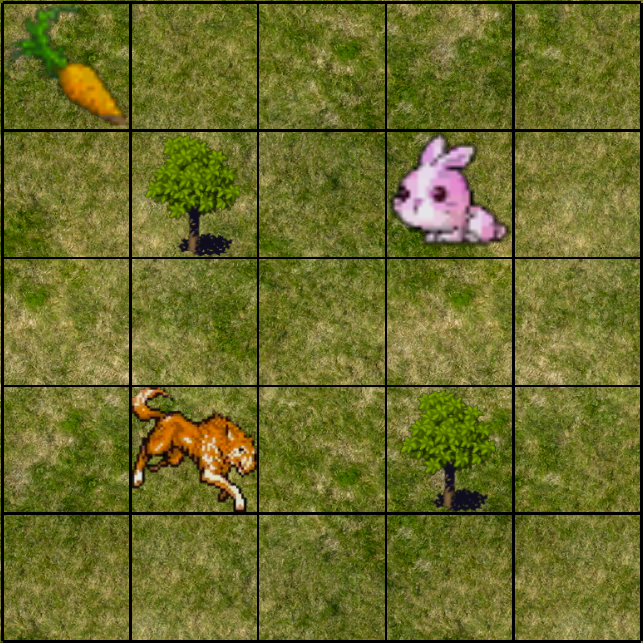
\includegraphics[height=2.4in]{bunny.png}
\end{center}


\caption{In the grid world above, the bunny must pursue two goals
  simultaneously: find food and avoid the wolf.  The bunny may move
  north, south, east, or west.  When it finds food it consumes the
  food and new food appears elsewhere in the grid world, when it meets
  the wolf it is eaten and ``dies.''}
\label{fig:bunny-picture}
\end{figure}

In this task each programmers wrote an agent that controls a bunny character in a simple world, depicted in Figure~\ref{fig:bunny-picture}.  The bunny world works as follows:

\begin{itemize}

\item The bunny world is a discrete grid of cells.  The bunny, wolf, and food each occupy one cell.

\item During each time step the bunny may move north, south, east, or west -- this is the bunny agent's action set.

\item Every two time steps the wolf moves towards the bunny.

\item If the bunny moves to the cell currently occupied by the food, the bunny eats the food, receives a signal from the simulation that it has eaten the food, and new food appears elsewhere.

\item If the wolf moves to the cell currently occupied by the bunny it eats the bunny and the episode ends.

\end{itemize}

Each programmer's Scala bunny and AFABL bunny were run for The simulation run, keeping track of how much food the bunny eats and how many times the bunny is eaten by the wolf.  Programmers will be asked to write bunny agents that live as long as possible and eat as much food as possible.

\subsection{Task 2: Mating Bunny}\label{sec:task2}

In this task each programmer will write a bunny agent for a world that is identical to the world in Task 1 except that the bunny must also find mates.  The world will include one static  potential mate that behaves similarly to the food.  When the bunny finds the potential mate, the bunny receives a signal that it has ``mated,'' the mate disappears, and another potential mate appears elsewhere.  The simulation runs as in Task 1, additionally keeping track of how many mates the bunny finds.  As in Task 1, programmers will be asked to write bunny agents that live as long as possible, eat as much food as possible, and find as many mates as possible.

%% \subsection{Task 3: Adding Wind, Spoiling Food, and Picky Mates}\label{sec:task3}

%% In this task each programmer will write a bunny agent for a world with the same elements as in Task 2 and with the same goals for the bunny, but the world is more complex.  In particular:

%% \begin{itemize}

%% \item There is constant wind from an unchanging direction that affects the wolf's ability to find the bunny.  The wolf will only move toward the bunny if the wolf is downwind of the bunny.

%% \item If food is not eaten within 15 time steps after it appears, it spoils.  Spoilage is represented by the food disappearing and new food appearing elsewhere.

%% \item To simulate selection of fit bunnies, potential mates will only accept the bunny if the bunny has eaten within 10 time steps (a hungry bunny is an unsuccessful bunny and therefore not fit for mating).  Rejection will be represented by the potential mate remaining in place and the bunny not receiving a signal that mating has occurred.

%% \end{itemize}

\section{Quantitative Results}

We analyzed the code submitted for each task to determine:

\subsection{Code Size}

How much code was required for each task with and without AFABL.

PLACEHOLDER PLACEHOLDER PLACEHOLDER PLACEHOLDER PLACEHOLDER PLACEHOLDER PLACEHOLDER PLACEHOLDER PLACEHOLDER PLACEHOLDER PLACEHOLDER PLACEHOLDER PLACEHOLDER PLACEHOLDER PLACEHOLDER PLACEHOLDER PLACEHOLDER PLACEHOLDER PLACEHOLDER PLACEHOLDER PLACEHOLDER PLACEHOLDER PLACEHOLDER PLACEHOLDER PLACEHOLDER PLACEHOLDER PLACEHOLDER PLACEHOLDER PLACEHOLDER PLACEHOLDER PLACEHOLDER PLACEHOLDER PLACEHOLDER PLACEHOLDER PLACEHOLDER PLACEHOLDER PLACEHOLDER PLACEHOLDER PLACEHOLDER PLACEHOLDER PLACEHOLDER PLACEHOLDER PLACEHOLDER PLACEHOLDER PLACEHOLDER PLACEHOLDER PLACEHOLDER PLACEHOLDER PLACEHOLDER PLACEHOLDER PLACEHOLDER PLACEHOLDER PLACEHOLDER PLACEHOLDER PLACEHOLDER PLACEHOLDER

\subsection{Time}

Time spent on Scala bunny versus AFABL bunny.

PLACEHOLDER PLACEHOLDER PLACEHOLDER PLACEHOLDER PLACEHOLDER PLACEHOLDER PLACEHOLDER PLACEHOLDER PLACEHOLDER PLACEHOLDER PLACEHOLDER PLACEHOLDER PLACEHOLDER PLACEHOLDER PLACEHOLDER PLACEHOLDER PLACEHOLDER PLACEHOLDER PLACEHOLDER PLACEHOLDER PLACEHOLDER PLACEHOLDER PLACEHOLDER PLACEHOLDER PLACEHOLDER PLACEHOLDER PLACEHOLDER PLACEHOLDER PLACEHOLDER PLACEHOLDER PLACEHOLDER PLACEHOLDER PLACEHOLDER PLACEHOLDER PLACEHOLDER PLACEHOLDER PLACEHOLDER PLACEHOLDER PLACEHOLDER PLACEHOLDER PLACEHOLDER PLACEHOLDER PLACEHOLDER PLACEHOLDER PLACEHOLDER PLACEHOLDER PLACEHOLDER PLACEHOLDER PLACEHOLDER PLACEHOLDER PLACEHOLDER PLACEHOLDER PLACEHOLDER PLACEHOLDER PLACEHOLDER PLACEHOLDER

\subsection{Cyclomatic Complexity}

PLACEHOLDER PLACEHOLDER PLACEHOLDER PLACEHOLDER PLACEHOLDER PLACEHOLDER PLACEHOLDER PLACEHOLDER PLACEHOLDER PLACEHOLDER PLACEHOLDER PLACEHOLDER PLACEHOLDER PLACEHOLDER PLACEHOLDER PLACEHOLDER PLACEHOLDER PLACEHOLDER PLACEHOLDER PLACEHOLDER PLACEHOLDER PLACEHOLDER PLACEHOLDER PLACEHOLDER PLACEHOLDER PLACEHOLDER PLACEHOLDER PLACEHOLDER PLACEHOLDER PLACEHOLDER PLACEHOLDER PLACEHOLDER PLACEHOLDER PLACEHOLDER PLACEHOLDER PLACEHOLDER PLACEHOLDER PLACEHOLDER PLACEHOLDER PLACEHOLDER PLACEHOLDER PLACEHOLDER PLACEHOLDER PLACEHOLDER PLACEHOLDER PLACEHOLDER PLACEHOLDER PLACEHOLDER PLACEHOLDER PLACEHOLDER PLACEHOLDER PLACEHOLDER PLACEHOLDER PLACEHOLDER PLACEHOLDER PLACEHOLDER

\section{Qualitative Results}

Programmers responded to a questionnaire to give their impressions of agent programming in AFABL versus agent programming in Scala.

\begin{enumerate}
\item I have a positive impression of agent programming in Scala.

Rationale: programmers’ impression of Scala will provide a baseline for evaluating
programmers’ impression of AFABL.

\item I found it easier to write the agents using AFABL’s programming constructs compared to bare Scala.

Rationale: the point of AFABL is to facilitate agent programming, so programmers should have a more positive impression of AFABL for agent programming.

\item I believe that AFABL facilitated more reusable and maintainable code for agents compared to bare Scala.

Rationale: answers to this question should correlate with answers to Question 1.

\item If given the choice, I would choose AFABL over Scala for agent programming projects.

Rationale: answers to this question should correlate with answers to Question 2.

\item I found it easier to use AFABL compared to Scala for Task 1.

  Rationale: in addition to objective analyses of task submissions, we want to know whether programmers subjectively prefer AFABL.

\item What was it about AFABL that made the Task 1 easier or harder?

Rationale: we want to get open-ended feedback for things we didn’t anticipate.

\item I found it easier to use AFABL compared to Scala for Task 2.

Rationale: in addition to objective analyses of task submissions, we want to know whether programmers subjectively prefer AFABL.

\item What was it about AFABL that made the Task 2 easier or harder?

\end{enumerate}

\section{Discussion}

\subsection{Authorability and the Agent Programming Space}

Authorability is the ease with which a programmer can author the behavior of agents.  Concretely, we suggest a framework for assessing authorability that considers domain knowledge requirements, algorithm knowledge requirements, and the adaptability of agents.

{\bf Domain knowledge} refers to the world-specific details the agent author must program into the agent for a particular domain.  Examples of domain knowledge include representations of state and the dynamics of the world, that is, how actions cause transitions from one state to another.

{\bf Algorithm knowledge} refers to the degree of algorithm detail that must be programmed in the agent.  An agent using a general-purpose programming language with no libraries to support agent programming would need to write the agent's behavior algorithms from scratch. Even an agent using an agent programming library would still likely need to encode a significant amount of algorithm knowledge in the agent. For example, an agent agent that uses a STRIPS planner for action selection would need to contain details of STRIPS operators and the mechanisms for selecting them in response to state perception.

{\bf Adaptability} refers to the ease with which an agent, once authored, can adapt to a changing world or be reused in a different world.

These factors are not completely orthogonal.  High domain knowledge requirements can hinder adaptability because agent agents need to be preprogrammed for worlds that have different dynamics.  Domain knowledge and algorithm knowledge often go hand-in-hand, for example in the encoding of heuristic functions.  Returning to our STRIPS example, STRIPS operators essentially encode world dynamics into the decision making algorithm, thereby coupling domain knowledge and algorithm knowledge.

We say that authorability is high when required domain knowledge is low, algorithm knowledge is low, and adaptability is high.  Such an agent is easy to program in the first place, can adapt to a world with non-stationary dynamics, and can be reused in new worlds with minimal reprogramming.

With this working framework for assessing the authorability of agent programming approaches we can map the agent programming space as a spectrum from fully scripted to fully learning approaches.

\subsubsection{Fully scripted agent Programming}

Fully scripted agents are the most common type of agents.  The scripts that control such agents specify every detail of the agent's behavior ahead of time.  While scripted agents can pursue goals and exhibit intelligence, the manner in which these goals are pursued must be written explicitly by the agent author, and if these goals are to be pursued using a particular algorithm, such as a planning algorithm, the algorithm itself must be encoded (or used as a library) from within the code.

In terms of our authorability framework, fully scripted agents have the
following properties.
\begin{itemize}
\item Domain knowledge: high. A fully scripted agent must specify a knowledge representation for perception and action that facilitates all the kinds of analyses and decisions the agent will make.  The dynamics of the world must be known in advance and encoded in he script to allow the agent to pursue goals.
\item Algorithm knowledge: high.  Although the algorithms may be simple, such as big if-else ladders, the agent author must have complete knowledge of how the agent's behavior algorithms work.  More complex algorithms mean more complex knowledge for the agent author to manage, fully scripted approaches scale poorly to more complex agents.
\item Adaptability: low.  Once an agent is fully scripted for a given environment, it must be reprogrammed for new environments with different dynamics.  Also, any run-time adaptivity must be scripted explicitly.
\end{itemize}

\subsubsection{Fully Machine Learning agent Programming}

\begin{itemize}
\item Domain knowledge: low. With a sufficiently abstract state
  representation, the agent can have very little domain knowledge.
\item Algorithm knowledge: low to moderate.  The choice of machine
  learning algorithm and state representation determine the level of
  algorithm knowledge necessary to author a fully machine learning
  agent.
\item Adaptability: high.  Adaptability is the key advantage of
  machine learning.
\end{itemize}

Neither of these two endpoints of the agent authorability spectrum is desirable.  Fully scripted agents are laborious to write.  Fully machine learning agents typically exhibit a long period of decreasing incompetence until their learning algorithms have sufficient data.  What we want is something in between fully scripted and fully machine learning agents.


{\bf Finding the NPC Authorability Sweet Spot with AFABL}

AFABL's integrated reinforcement learning separates the dynamics of the world from the action-slection logic in the agent, freeing the programmer from writing domain-dependent code and facilitating the adaptation of agents to new worlds.

\begin{itemize}
\item Domain knowledge: as much or as little as you want.  You can program the parts you know how to program, and leave AFABL to learn the rest automatically.
\item Algorithm knowledge: moderate.  AFABL is based on the agent and
  reinforcement learning models.  Behaviors are programmed as actions
  that execute in response to observed state (hence ``behavior''), and
  automatic behaviors additionally specify reward signals that enable
  AFABL to learn the best responses to particular states.
\item Adaptability: high.
\end{itemize}


\subsection{Contributions}

\begin{itemize}
\item AFABL, an adaptive agent programming framework/DSL that integrates MRL into the Scala language.
\item Idioms and design patterns for using AFABL to program adaptive agents.
\item Exploratory knowledge on the kinds of framework/language features and debugging tools that are useful in adaptive partial-programming, the roles they play in the development process, and the benefits they provide.
\item Confirmatory knowledge that a programming language integrating MRL provides measurable adaptivity benefits for appropriate agent programming problems.
\end{itemize}
